%
% Lexical Disambiguation
%

\subsection{Sentential Context}
In the previous section, we showed how weakened PFC/DA interactions can hinder the integration of information over time. Such temporal integration is also important for determining the meaning of ambiguous words in a sentence. Homographs are words that share spelling but have different meanings and pronunciations (e.g., ``bow'', ``tear''). To identify the word referenced by a homograph, we typically must rely on sentential context. People with autism have difficulties utilizing context when interpeting homographs. Instead, they tend to produce the most frequent pronunciation~\cite{HappeF:1997:WCCHomographs}. Some neurocomputational models of sentence processing use an SRN architecture, like that used to model the SRTT. The context layer integrates a sequence of words into an evolving representation of the sentence. As before, the SRN must update the context layer in a fast and appropriate manner in order to integrate information from the full sequence of words.

\subsection{Lexical Ambiguity in Schizophrenia}
Interestingly, people with schizophrenia also have problems utilizing context in language disambiguation tasks~\cite{CohenJD:1992:Schizophrenia}. The specific pattern of deficits is different than those observed in ASD, however. Coarsely, schizophrenics lose context with delay, while people with autism often fail to use sentential context even when that information was recently provided.

Also, there is evidence that many schizophrenia symptoms arise from abnormal DA functioning~\cite{CohenJD:1992:Schizophrenia}. How might the DA dysfunctions in schizophrenia and autism differ so as to produce observed differences in lexical disambiguation? One possibility involves the differential effects of ``tonic'' DA, which changes slowly in cortex, and ``phasic'' DA, which rapidly influences processing. Cohen and Servan-Schreiber (1992) argue that schizophrenia symptoms arise from abnormal tonic DA levels. In contrast, it is phasic DA signaling that is thought to capture TD Error, as in adaptive gating models of PFC. This leads to the hypothesis that degraded PFC updating, as in the SRTT model, should produce ASD-like patterns of disambiguation deficits, while degraded active maintenance of PFC representations should result in the error pattern seen in schizophrenia.

\subsection{Testing Context Sensitivity}
There is a psychological test has been used to evaluate both people with schizophrenia and ASD on their ability to utilize context when disambiguating words~\cite{CohenJD:1992:Schizophrenia,HappeF:1997:WCCHomographs}. The test uses ambiguous words with both a high frequency interpretation and a low frequency one. On each trial, a sentence fragment is presented which contains one ambiguous word (e.g., ``with a BOW'') along with a disambiguating fragment (e.g., ``the juggler ended his act''). The sentence fragments are presented in various orders. Specifically, there are four conditions: (1) the low frequency meaning is correct and the context comes last, (2) the low frequency meaning is correct and the context comes first, (3) the high frequency meaning is correct and the context comes first, and (4) the high frequency meaning is correct and the context comes last.

People with autism demonstrate problems identifying the contextually appropriate meaning of the ambiguous word in both conditions (1) and (2), providing a significantly higher percentage of incorrect high frequency responses compared with typically developing controls~\cite{HappeF:1997:WCCHomographs}. (See Figure~\ref{asd-lexamb-study}.) ASD participants show no significant differences from controls in conditions (3) and (4). The profile for schizophrenics is slightly different. People with schizophrenia show an impairment in utilizing context, but only during condition (2), when the context is presented first. (See Figure~\ref{schiz-lexamb-study}.) This has been interpreted as evidence for problems maintaining contextual information over time in schizophrenia. (Condition (4) was not tested in the schizophrenic population, so no human data are available in that case.)
%To clarify, this suggests that in condition (1), the contextual information was temporally close enough to the required response to enable the subjects diagnosed with schizophrenia to correctly utilize this information and make a proper response.  Condition (4) was not tested in the schizophrenic population, and therefore no human data is available.  

\begin{figure}[tp]
\begin{center}
	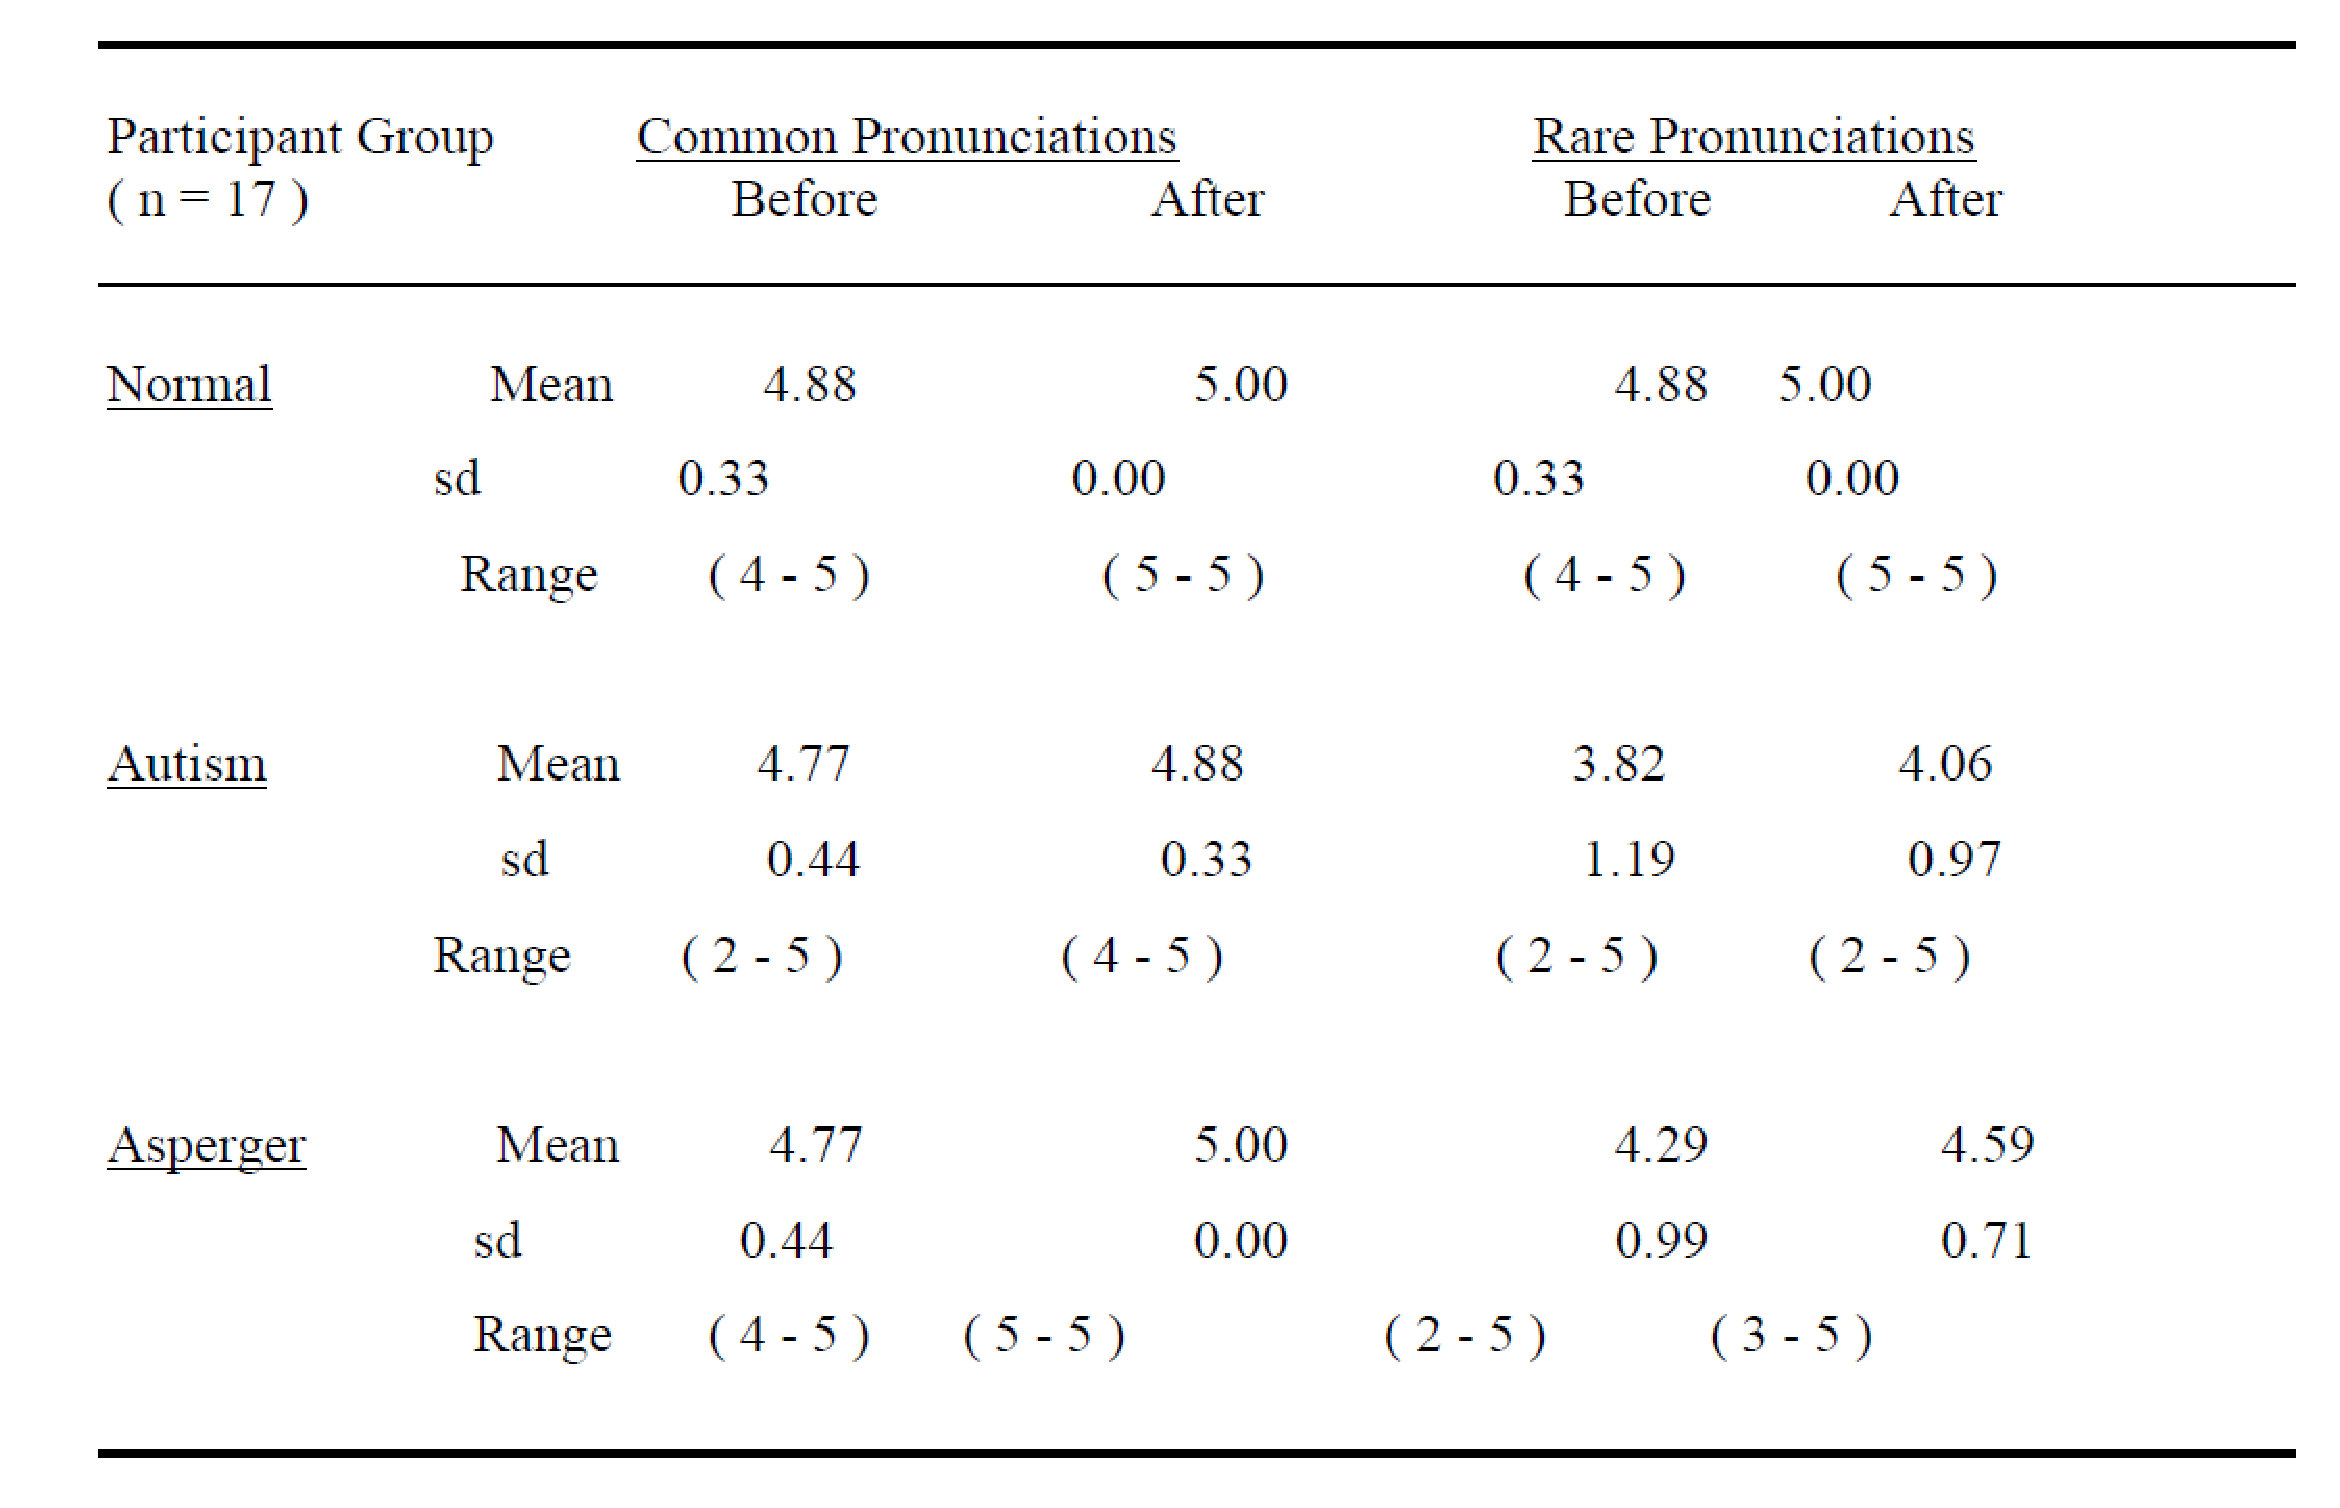
\includegraphics[width=115mm]{figures/asd_lexamb_study_results.eps}
\end{center}
\caption{Lexical Disambiguation in ASD. ``Common'' refers to the high frequency interpretation of the ambiguous word being appropriate, while ``Rare'' refers to cases in which the low frequency interpretation is correct. ``Before/After'' refers to the order of sentence fragments, with the ambiguous word occurring before/after the contextual information, respectively. Table reproduced from Jolliffe and Cohen (1999).}
\label{asd-lexamb-study}
\end{figure} 

\begin{figure}[tp]
\begin{center}
	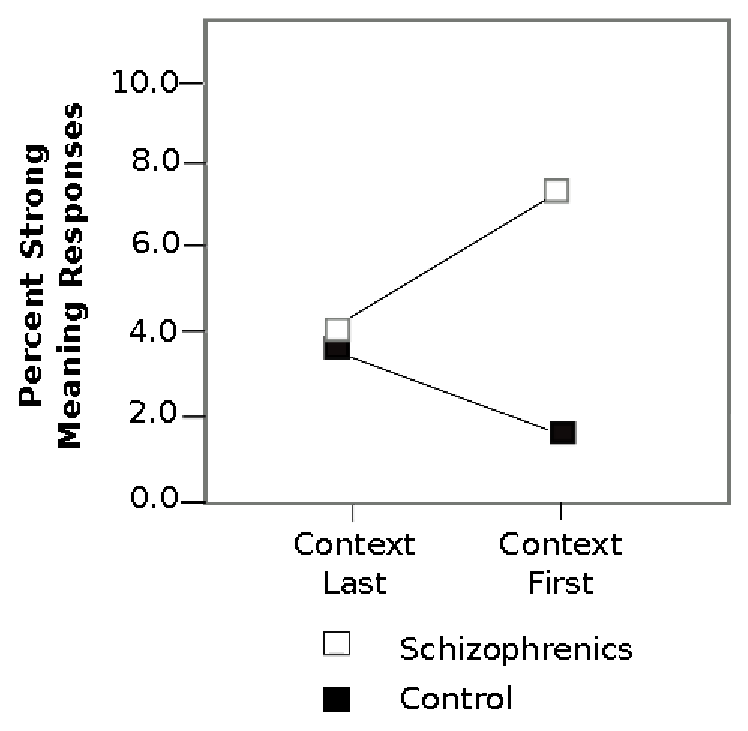
\includegraphics[width=100mm]{figures/schiz_lexamb_study_results.eps}
\end{center}
\caption{Lexical Disambiguation in Schizophrenia. Vertical axis shows percentage of errors using the most common interpretation of the ambiguous word, when the rare interpretation was correct. Figure adapted from Cohen and Servan-Schreiber (1992).}
\label{schiz-lexamb-study}
\end{figure} 

\subsection{Modeling Lexical Disambiguation}
The connectionist model utilized by Cohen and Servan-Schreiber (1992) was modified to investigate lexical disambiguation in people with autism and schizophrenia. (See Figure~\ref{cohen-servan-schreiber-model}.)  A localist code was used to represent words as inputs to the network. These inputs included ambiguous words and words that could act as contextual cues. The output of the network (the ``Meaning Output Module'' in Figure~\ref{cohen-servan-schreiber-model}) also used a localist code to represent the various possible meanings of the current word being presented to the network. For example, separate output units would be used to represent the meaning of ``BANK'' as a ``financial institution'' and the meaning of ``BANK'' as ``land alongside a river''.

\begin{figure}[tp]
\begin{center}
	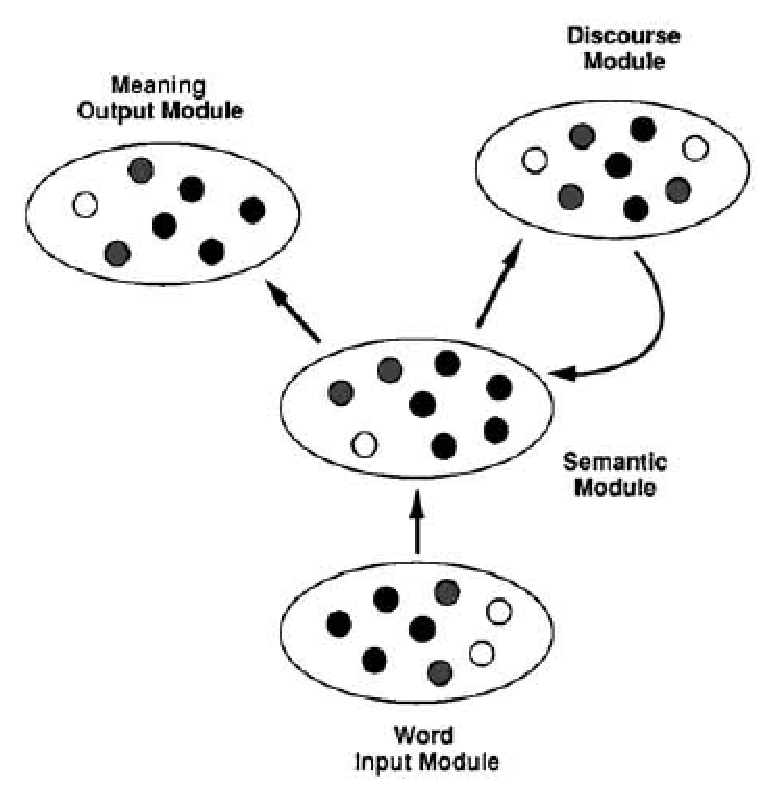
\includegraphics[width=100mm]{figures/Cohen_ServanSchreiber_Model.eps}
\end{center}
\caption{The Original Lexical Disambiguation Model. Image adapted from Cohen and Servan-Schreiber (1992).}
\label{cohen-servan-schreiber-model}
\end{figure} 

While, in the original model, the context layer (``Discourse Module'' in Figure~\ref{cohen-servan-schreiber-model}) used a researcher specified code for sentential context information, we allowed this layer to learn its own distributed representations by training the network as an SRN on the task of producing the correct output meaning for each input word form, in the context of previously presented inputs. Specifically, there were 100 input units encoding 50 ambiguous words and 50 disambiguating context words. The output contained two units for each of two meanings of the 50 ambiguous words, plus 50 units for the meanings of the context words, for a total of 150 output units. Of the two meanings for each ambiguous word, one was considered ``strong'' (high frequency), and the second was considered ``weak'' (low frequency). The hidden and context layers contained 100 units, though varying this value had little effect.

Each trial consisted of presenting the model with a sequence of three words, with the model expected to output the appropriate meaning of each word as it was presented. Each sequence began with a context/ambiguous word pair, with the order of these two words counterbalanced to produce ``Context Presented First'' trials and ``Context Presented Last'' trials. The third word in each sequence was a repetition of the ambiguous word, with the model expected to produce the context appropriate meaning for this probe word regardless of the order of the initial word pair. During SRN training, the strong word meaning was used on $70\%$ of trials, and the weak meaning was used on $30\%$ of trials. On every trial, the context word perfectly disambiguated the otherwise ambiguous word. (See Figure~\ref{lexamb-model-task}.) 

%The corpus used for training involved 50 input units representing 50 ambiguous homographs as well as 50 disambiguating context word units.  Two context units were associated with each of the 50 homograph units. Also, each context unit is paired with two different homograph units, ensuring that every context unit is involved in two completely different disambiguation trials.  This prevents the network from learning a one-to-one association of a context unit to a specific homograph word meaning, removing any possibility that the network could solve the task while ignoring all of the homograph units, instead relying only the contextual information.  One context unit represented the more frequent use (strong) and one unit for the less frequent (weak) use of each homograph.  This resulted in 150 possible outputs for the network (100 possible homograph interpretations and 50 context words).  Each output can be thought of as representing the proper ``meaning'' input words presented to the network.  (See Figure~\ref{lexamb-model-task}.)  %The network also used 100 units each within the Hidden layer and the Context Layer, it should be noted, however, that varying this value had little effect on the networks overall performance.

% One word is presented to the network at a time, requiring the network to make a response to every word regardless of type.  On each trial, the network is presented with a mini-clause consisting of three words, including a context/homograph pair followed by a homograph probe. The pieces of each mini-clause represent the sentences presented to the subjects in the original studies, followed by questioning the subjects on the meaning of the ambiguous word (the probe).  The order of presentation for the context and homograph units were counterbalanced, ensuring equal experience with utilizing context at both the beginning and the end of mini-clauses.  The final probe homograph unit was always presented last, and was needed to assess if the network could properly disambiguate the meaning of the homograph. The network was presented with the strong interpretation of the homographs on 70\% of the trials and the weak interpretation on 30\%.

After training, the network was tested on the same three word sequences on which it was trained, following the procedure used by Cohen and Servan-Schreiber (1992) without modification. The primary measure of interest was the fraction of trials in which the model output the strong meaning during the final probe word presentation in the sequence, but the weak meaning was contextually appropriate.

\begin{figure}[tp]
\begin{center}
	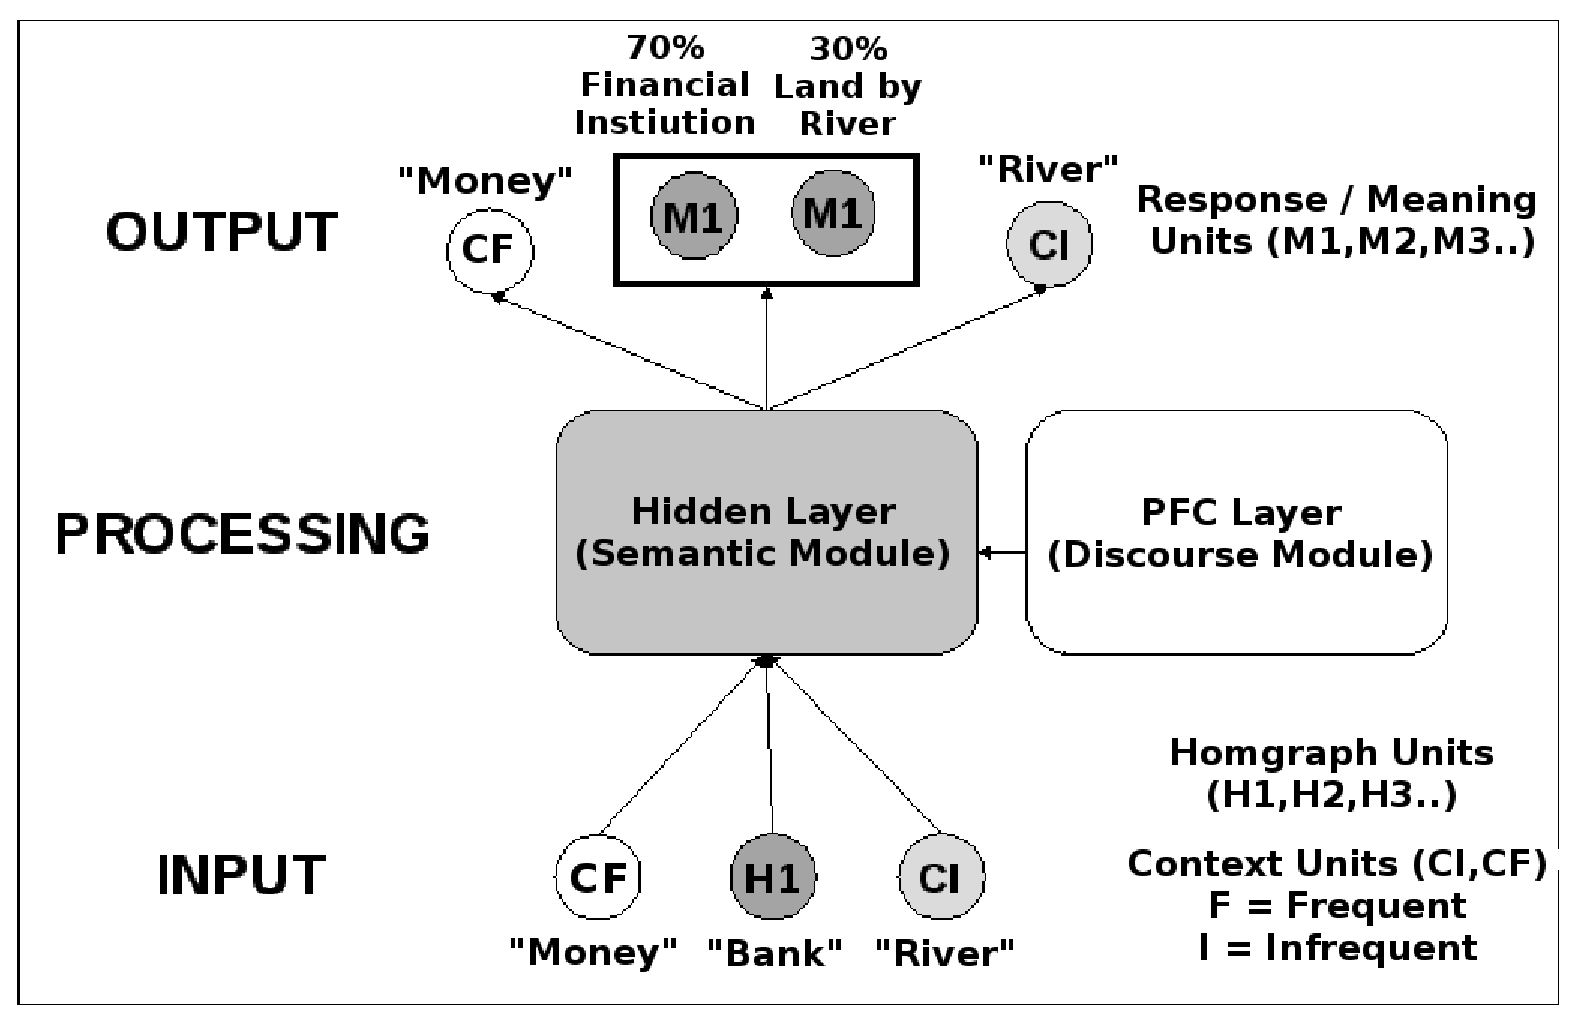
\includegraphics[width=115mm]{figures/lexAmb_network_cartoon.eps}
\end{center}
\caption{Lexical Disambiguation Model and Task.  The task was to correctly respond to any input word by activating the output unit encoding the appropriate meaning for that word. The context units were used to retain sentential context, needed for disambiguation.}
\label{lexamb-model-task}
\end{figure} 

\subsection{Modeling Schizophrenia}
In the original model of schizophrenic performance, Cohen \& Servan-Schreiber implemented their hypothesized reduction in tonic DA levels by reducing the gain of the activation function on all modeled PFC units. Coupled with the dynamics of the network, the result was a less stable PFC representation of context. Thus, presenting disambiguating context early could result in the gradual loss of information needed to determine the correct meaning of the probe. This manipulation successfully matched the pattern of behavior seen in schizophrenia. We approximated the gain reduction used in the original model by decaying context layer activation by a fixed multiplicative constant. In our model of healthy performance, $30\%$ of context layer activity was retained on each time step. To model schizophrenia at various levels of severity, this context maintenance parameter was reduced to $20\%$, $10\%$, and $0\%$. Since schizophrenic symptoms typically appear after a substantial amount of development, the context activation decay was only instantiated after the model had completed its SRN training.

%By systematically reducing the parameter that controls the amount of previous Context Layer activity retained from time step to time step, we can functionally reduce the stability of the contextual representations maintained within the modeled PFC.  This manipulation provides an extremely close approximation to the gain reduction performed by Cohen \& Servan-Schreiber.   Also, schizophrenia most often emerges after a significant amount of development has occurred, therefore this deficit was only instantiated after the network had been trained to criterion.  In the healthy model, the context maintenance parameter is set to ensure that 30\% percent of the previous Context Layer's activation was retained from the previous time step.  In order to investigate schizophrenic behavior we reduced this parameter to 20\%, 10\%, and 0\%, systematically destabilizing the modeled PFC. 
%Under normal circumstances, the Context Layer has the ability to effectively hold onto previous information over multiple time steps.  In a standard SRN, a complete copy of the previous time steps Hidden Layer activity pattern is copied directly into the Context Layer upon every time step.  However, within the Leabra framework there are two mixing parameters responsible for allocating what percentage of the activation is a pure copy of the previous Hidden Layer activity and what percentage is maintained from the previous state of the Context Layer itself.  These parameters can be seen as manipulating how well the network updates the contents of the PFC and how well the network can actively maintain this information within the PFC respectively.  By systematically reducing the parameter that controls the amount of previous Context Layer activity retained from time step to time step, we can functionally reduce the stability of the contextual representations maintained within the modeled PFC.  This manipulation provides an extremely close approximation to the gain reduction performed by Cohen \& Servan-Schreiber.   Also, schizophrenia most often emerges after a significant amount of development has occurred, therefore this deficit was only instantiated after the network had been trained to criterion.  In the healthy model, the context maintenance parameter is set to ensure that 30\% percent of the previous Context Layer's activation was retained from the previous time step.  In order to investigate schizophrenic behavior we reduced this parameter to 20\%, 10\%, and 0\%, systematically destabilizing the modeled PFC Layer's maintained pattern of activity. 

%\begin{figure}[tp]
%\begin{center}
%	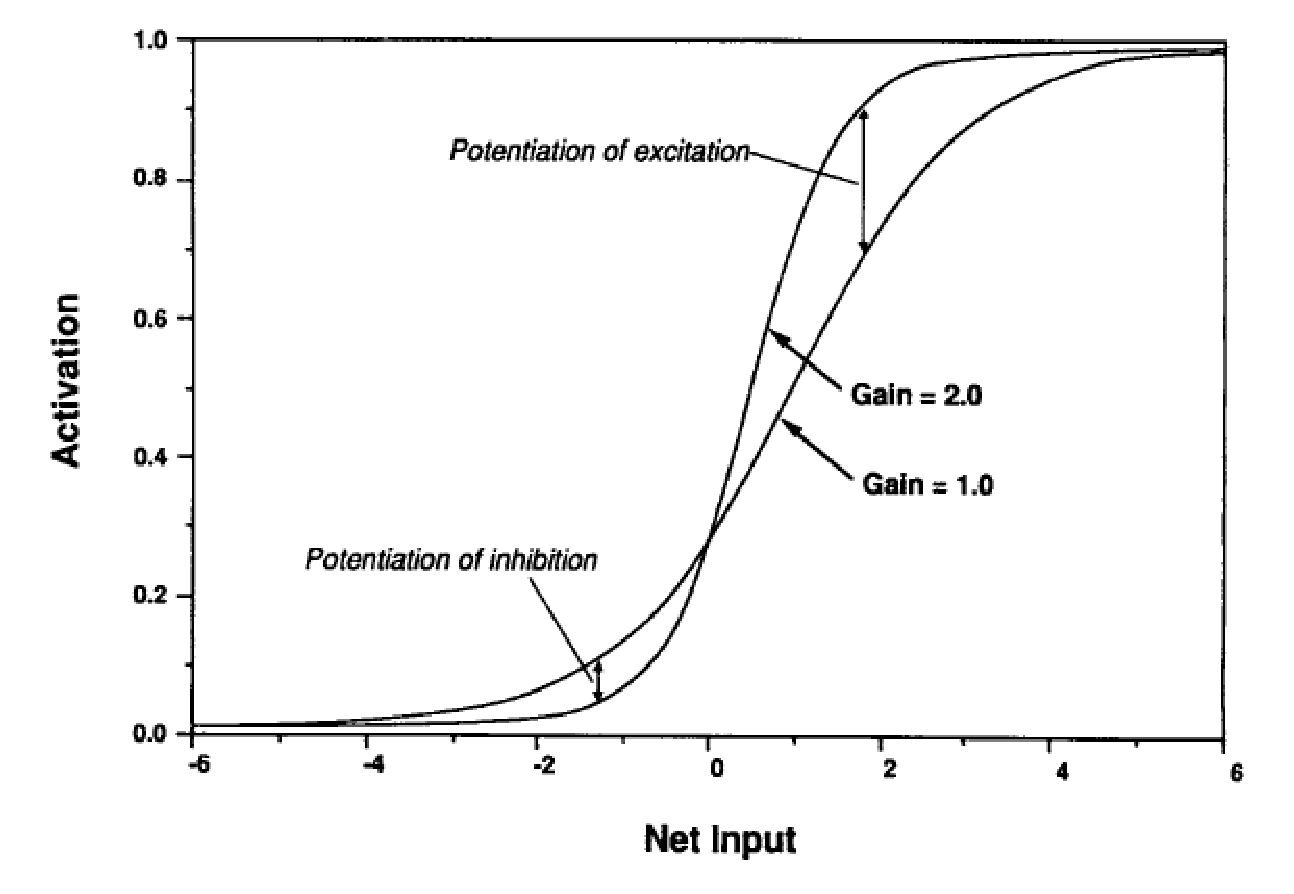
\includegraphics[width=100mm]{figures/gain_manipulation.eps}
%\end{center}
%%\caption{Modeled effects of tonic DA on a standard activation function. An increase in the amount of DA heightens the effects of the net input, effectively increasing the signal-to-noise ratio in the network, while lower DA decreases the effects, reducing the signal-to-noise ratio. Image adapted from Cohen and Servan-Schreiber (1992).}
%\label{gain-manipulation}
%\end{figure} 

\subsection{Modeling Autism}
%In order to model the performance of people with autism, we propose to hinder the updating of the SRN context layer of the network as discussed previously.  Specifically, two distinct manipulations will be tested.  The first method will consist of gaussian noise being injected directly into the context layer of the SRN, resulting in contextual information which has been corrupted to varying degrees, based upon the amount of noise utilized.  In the second manipulation we will titrate the probability that the context layer is updated, mimicking a deficit flexible updating of the contents contained within the PFC.  This manipulation of the model is consistent with my proposed theory of impaired input and output gating of representations maintained within the PFC driven by DA interactions.  Importantly, this deficit will be instantiated from the beginning of development.  This is different than the modeled deficit proposed in Schizophrenia by Cohen and Servan-Schreiber, where the DA manipulation occurs after the task has been learned.   By instantiating a deficit in the context layer, the model may not be able to rely on temporally distant information, and, instead, must use the statistical regularities that are available at each time step.  The result should create a response bias towards the more frequently experienced words and a general inability to utilize context, as is observed in people with autism.

In order to model the performance of people with autism, we restricted the probability of successfully updating the context layer (PFC) upon each input presentation. Specifically, we investigated successful PFC updating probabilities of $100\%$ (healthy control), $90\%$, and $80\%$. The reduction of this probability made the temporally extended information in PFC less reliable, hindering the learning of appropriate use of sentential context. To capture the developmental nature of autism, we restricted updating of the modeled PFC layer from the beginning of SRN training.

\subsection{Simulation Results}

Model simulations were repeated 10 times in each of the experimental conditions, with initial synaptic weights randomized for each repetition, and results were aggregated over these 10 repetitions. The possible word triplets were presented in a random order during training, and synaptic strengths were not allowed to change during testing. We measured the number of errors committed when assigning a meaning to an ambiguous probe.

The schizophrenia model qualitatively matched the behavioral data and reproduced the seminal modeling results of Cohen \& Servan-Schreiber (1992). (See Figure~\ref{Schiz-Amb-Results}.) Control networks performed well regardless of the frequency of the correct meaning (``Rare'' vs.\ ``Common''). Also, the ordering of contextual information had virtually no effect on healthy model performance. However, as the PFC representations were systematically destabilized in order to model schizophrenia, the error rate rose significantly. Importantly, this increase in error only occurred when the context was presented first, but not when the context was presented last. 
%Two-way ANOVAs were performed separately on each destabilization level -- 0\% Destabilized (Control), 33\% Destabilized, 66\% Destabilized, and 100\% Destabilized --, with frequency (``Rare'' vs. ``Common'') and ordering (``Context First'' vs. ``Meaning First'') as factors.  An effect of frequency was observed as the PFC was destabilized 33\%, 66\%, and 100\% (respectively, F(1,36) = 18.29, p $< .05$; F(1,36) = 57.48, p $< .05$; F(1,36) = 78.98, p $< .05$).  Also, an effect of ordering was observed for each condition (respectively, F(1,36) = 14.97, p $< .05$; F(1,36) = 77.72, p $< .05$; F(1,36) = 109.42, p $< .05$). Importantly, a there was a significant frequency by ordering interaction effect in all cases where the PFC was destabilized (respectively, F(1,36) = 11.99, p $< .05$; F(1,36) = 54.84, p $< .05$; F(1,36) = 73.49 p $< .05$).  This supports the observation that only the context first error rate rose significantly as a result of PFC destabilization. No effects were found in the control network results for either frequency F(1,36) = .64, p $>.05$; or ordering F(1,36) = 3.47, p $>.05$, and the frequency by ordering interaction was also non-significant F(1,36) = 1.77, p $>.05$.  This matches patterns of behavior reported in previous schizophrenia research~\cite{CohenJD:1992:Schizophrenia}, which demonstrated that people with schizophrenia have difficulty utilizing context when it is presented temporally distal from the homograph it is intended to disambiguate.    
%Two-way ANOVAs were performed separately on each destabilization level -- 0\% Destabilized (Control), 33\% Destabilized, 66\% Destabilized, and 100\% Destabilized --, with frequency (``Rare'' vs. ``Common'') and ordering (``Context First'' vs. ``Meaning First'') as factors.  An effect of frequency was observed as the PFC was destabilized 33\%, 66\%, and 100\% (respectively, F(1,36) = 18.29, p $< .05$; F(1,36) = 57.48, p $< .05$; F(1,36) = 78.98, p $< .05$).  Also, an effect of ordering was observed for each condition (respectively, F(1,36) = 14.97, p $< .05$; F(1,36) = 77.72, p $< .05$; F(1,36) = 109.42, p $< .05$). Importantly, a there was a significant frequency by ordering interaction effect in all cases where the PFC was destabilized (respectively, F(1,36) = 11.99, p $< .05$; F(1,36) = 54.84, p $< .05$; F(1,36) = 73.49 p $< .05$).  This supports my observation that only the context first error rate rose significantly as a result of PFC destabilization. No effects were found in the control network results for either frequency F(1,36) = .64, p $>.05$; or ordering F(1,36) = 3.47, p $>.05$, and the frequency by ordering interaction was also non-significant F(1,36) = 1.77, p $>.05$.  This matches patterns of behavior reported in previous schizophrenia research~\cite{CohenJD:1992:Schizophrenia}, which demonstrated that people with schizophrenia have difficulty utilizing context when it is presented temporally distal from the homograph it is intended to disambiguate.    

By restricting the ability of the context layer (PFC) to appropriately update, the ASD model captured previously observed patterns of behavior~\cite{HappeF:1997:WCCHomographs}. (See Figure~\ref{ASD-Amb-Results}.) Specifically, as the probability of successful updating was reduced, the ASD networks became increasingly reliant on the frequency of word meanings. This manifested in higher error rates when the model needed to utilize contextual information, regardless of the temporal distance from the context to the probe, as seen in people with autism.
% (See Figure~\ref{asd-lexamb-study}.) 
%Two-way ANOVAs were performed separately on each level of PFC updating  -- 100\% probability to update PFC (Control), 90\% probability to update PFC, and 80\% probability to update PFC -- with frequency (``Rare'' vs. ``Common'') and ordering (``Context First'' vs. ``Meaning First'') as factors.  An effect of frequency was observed in the ``autistic-like'' condition, where the PFC is restricted to update only 90\% and 80\% of the time (respectively, F(1,36) = 64.52, p $< .05$; F(1,36)=116.58, p $< .05$). However, an effect of ordering was not observed (respectively, F(1,36) = 0.35, p $> .05$; F(1,36) = 0.31, p $> .05$). Also, the frequency by ordering interaction was not significant in either case (respectively, F(1,36) = 0.87, p $. .05$; F(1,36) = 0.31, p $> .05$). These results suggest that the model of autistic performance has difficulty utilizing contextual information to overcome a more frequent interpretation of a homograph, regardless of when it is presented in the sentence.  No effects were found in the control network results for either frequency F(1,36) = .64, p $>.05$; or ordering F(1,36) = 3.47, p $>.05$, and the frequency by ordering interaction was also non-significant F(1,36) = 1.77, p $>.05$.  It is important to note that as the probability of updating the Context Layer was reduced, the model of autistic behavior performed worse overall when compared to the control network, including common interpretations of the homographs.   This pattern was not reported in the behavioral study of people with ASD.  However, the extremely low number of sentences in each condition (5) may be resulting in ceiling effects, limiting the ability to reliably detect this difference in their sample. (See Figure~\ref{asd-lexamb-study}.) 

%\& Servan-Schreiber (1992). See Figures~\ref{Schiz-Amb-First} \& \ref{Schiz-Context-First}.)  The ``Control'' network performed well regardless of the frequency of the meaning word (``Rare'' vs.``Common'') as well as if the contextual information came early in the mini-clause(Context-First) or if it came later (Ambiguous-First).  However, as the PFC representations were systematically destabilized (as is hypothesized to occur in schizophrenia due to tonic-DA dysfunction), the error rate rose significantly for when the context was presented first, but not when the context was presented last.  This matches patterns of behavior reported in previous schizophrenia research~\cite{CohenJD:1992:Schizophrenia}
%Also, the model added to the original modeling effort by allowing the contextual representations in the modeled PFC be learned from experience, instead of being hand-coded by the modeler.

\begin{figure}[tp]
\begin{center}
	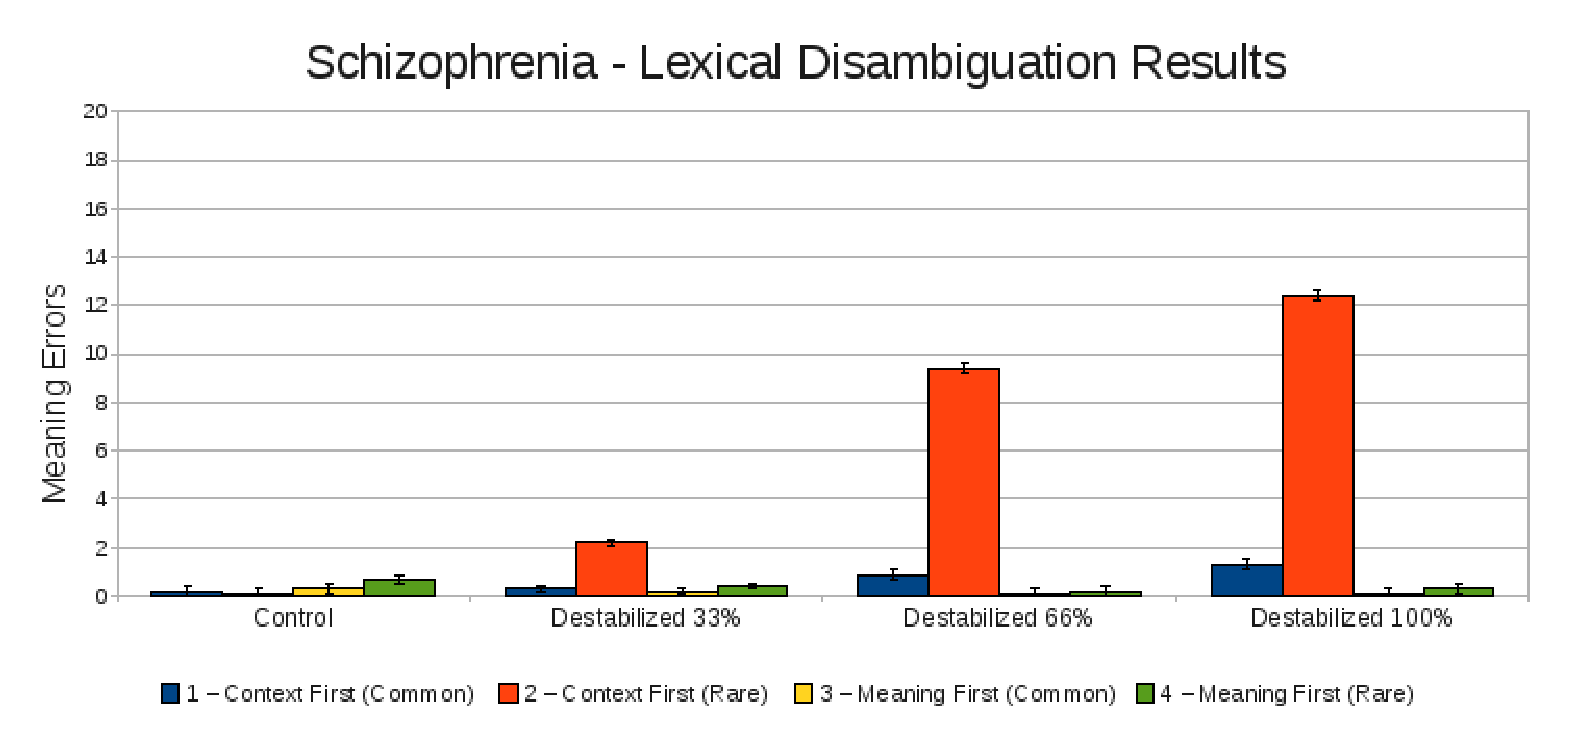
\includegraphics[width=140mm]{graphs/schiz_lexamb_results.eps}
\end{center}
\caption{Schizophrenia Model Results. As the modeled PFC is destabilized, the model performs selectively worse on condition (2).  In this condition, the contextual information is presented first and the model must use this information to override the more common interpretation of the ambiguous word.} 
\label{Schiz-Amb-Results}
\end{figure} 

\begin{figure}[tp]
\begin{center}
	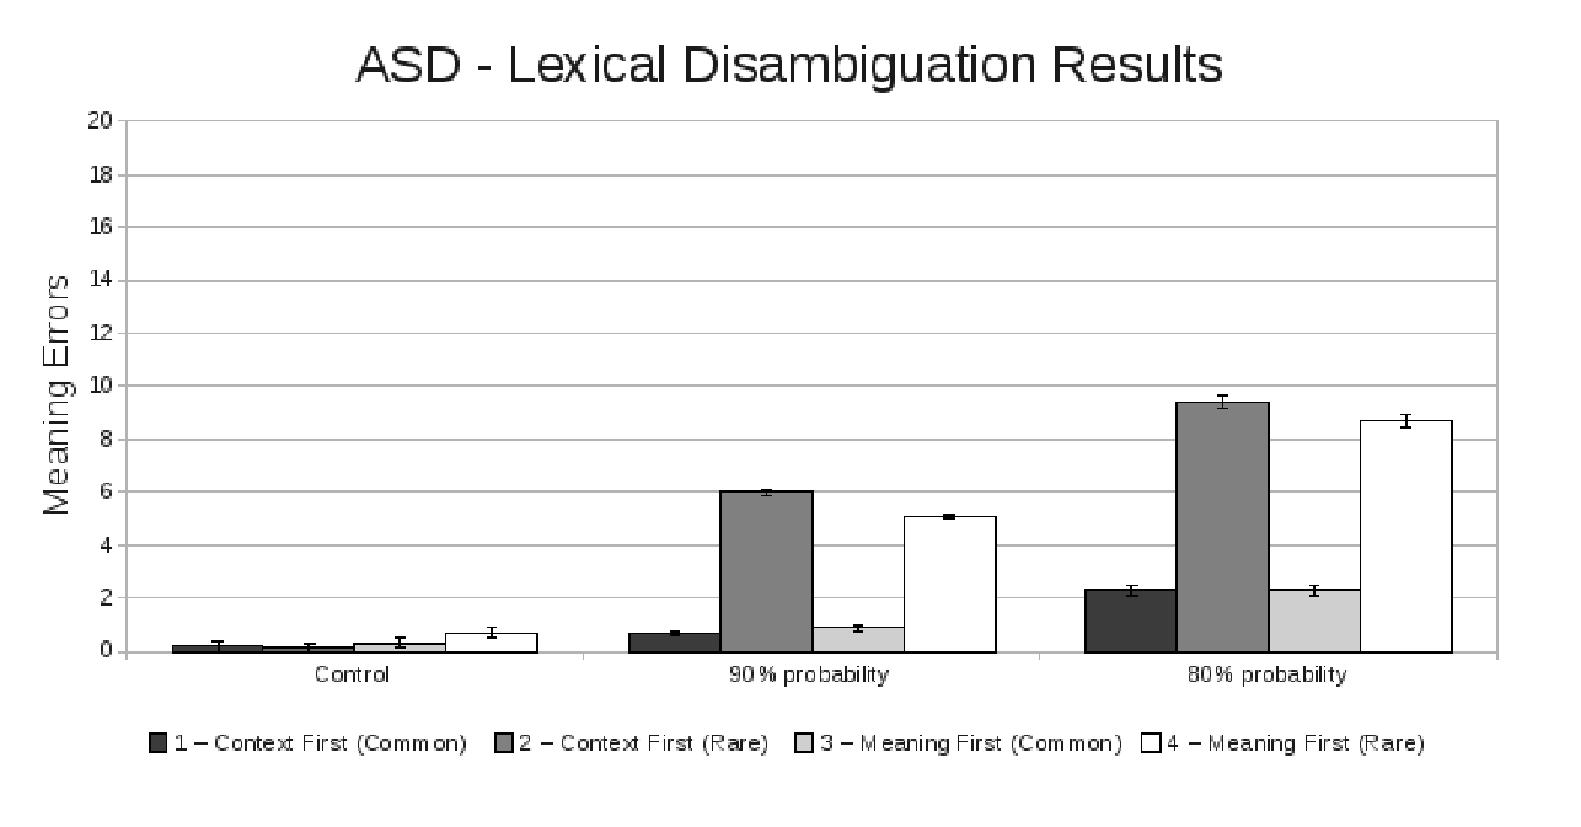
\includegraphics[width=140mm]{graphs/asd_lexamb_results.eps}
\end{center}
\caption{ASD Model Results. Systematically reducing the probability of PFC updating success resulted in worse performance on conditions (2) and (4). These are the conditions that require the use of contextual information in order to override the more common interpretation of the ambiguous word.} 
\label{ASD-Amb-Results}
\end{figure} 

\subsection{Summary}
%In this chapter modeling results were presented demonstrating how a specific neural difference, dysfunctional interactions between the mid-bran DA system and PFC, can capture patterns of dysfunction in people with autism when utilizing sentential context to disambiguate the meaning of homographs.  Our work suggests that improper DA / PFC interactions lead to problems flexibly updating the contents of the PFC, and difficulties arise due to the lack of reliable contextual representations.  This causes the model to rely more heavily on statistical regularities in the environment.  In other words, the model adopts a policy of responding with the most common interpretation of a homograph in order to minimize errors, in lieu of appropriate contextual guidance from the Context Layer.  A previously published and theoretically justified computational model of lexical disambiguation was modified in a manner consistent with my hypothesis in order to capture the behavior of people with autism~\cite{CohenJD:1992:Schizophrenia}.  Interestingly, the Cohen \& Servan-Schreiber model was originally developed as an investigation into lexical disambiguation difficulties in people with Schizophrenia.  This provided my investigation with an interesting clinical comparison group, especially considering the qualitatively different behavioral profiles of the two disorders coupled with the suggestion of DA dysfunction underlying each respective pattern.  By positing the disorders actually have different \emph{kinds of DA dysfunction}, namely tonic DA dysfunction in schizophrenia and phasic DA abnormalities in ASD, the model is capable of explaining both the original findings of Cohen \& Servan-Schreiber and the patterns of behavior found in people with ASD~\cite{JolliffeT:1997:Embedded,HappeF:1997:WCCHomographs}.  

Using a computational model very similar in structure to that used to capture SRTT performance in ASD, we have shown that dysfunction in the updating of PFC can explain deficits in word sense disambiguation observed in people with autism. The pattern of these deficits is distinct from that seen in schizophrenia, but the same model captures schizophrenic data by incorporating a reduction in PFC active maintenance stability, due to lower tonic DA levels.

